\documentclass[30pt,twocolumn,letterpaper]{article}
\usepackage{cvpr}
\usepackage{times}
\usepackage{booktabs}
\usepackage{epsfig}
\usepackage{graphicx}
\usepackage{amsmath}
\usepackage{amssymb}
\cvprfinalcopy
\def\cvprPaperID{****}
\def\httilde{\mbox{\tt\raisebox{-.5ex}{\symbol{126}}}}
\usepackage{graphicx}
\usepackage{indentfirst}
\setlength{\parindent}{2em}
\usepackage{cite}
\usepackage[colorlinks,linkcolor=red,anchorcolor=blue,citecolor=green,backref=page]{hyperref}
\author{Qilei Zhang\\\\
Jul 2 2018}
\title{Generative Visual Manipulation on the Natural Image Manifold}
\begin{document}
\maketitle
\begin{abstract}
  Realistic image manipulation is challenging because it requires modifying the image appearance in a user-controlled way, while preserving the realism of the result. Unless the user has considerable artistic skill, it is easy to fall off the manifold of natural images while editing.
\end{abstract}
\section{Introduction}
Visual communication is a sad one-sided nature. Generally, information is perceived by visual form, but only a few have enough talents to express themselves effectively. Even in the most mundane task, this imbalance will emerge\cite{Groen2012Low}. \\
\par
For most people, even simple image processing in PS image processing software is difficult to overcome. Any imperfect editor instantly makes the image totally unrealistic. In other words, the classic visual manipulation paradigm does not prevent users from shedding from natural images\cite{Nikolaidis2012Generative}.
\begin{figure}[htbp]
\small
\centering
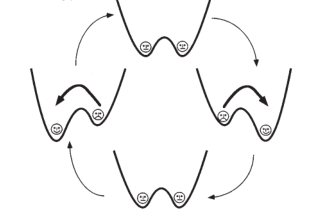
\includegraphics[width=20em]{000.png}
\caption{We use generative adversarial networks (GAN) to perform image editing
on the natural image manifold. We first project an original photo (a) onto a lowdimensional
latent vector representation (b) by regenerating it using GAN. We then
modify the color and shape of the generated image (d) using various brush tools (c)
(for example, dragging the top of the shoe). Finally, we apply the same amount of
geometric and color changes to the original photo to achieve the final result (e). See
our interactive image editing demo on Youtube.}
\label{fig:lable}
\end{figure}\\
\section{Prior Work}
Image editing is a recognized field in computer graphics, where input images are manipulated to achieve user specified specific targets. Examples of basic editing include global or partial change of the color property of an image. More advanced editing methods, such as image warpage or structured image editing, intelligently adjust the pixels in the image after user editing. When impressive results are made in the hands of experts, the results of these types of methods fail to look like real images.\\
\begin{figure}[htbp]
\small
\centering
\includegraphics[width=20em]{001.png}
\caption{GAN as a manifold approximation. (a) Randomly generated examples from a
GAN, trained on the shirts dataset; (b) random jittering: each row shows a random
sample from a GAN (the first one at the left), and its variants produced by adding
Gaussian noise to z in the latent space; (c) interpolation: each row shows two randomly
generated images (first and last), and their smooth interpolations in the latent space.}
\label{fig:lable}
\end{figure}\\
\par
Common artifacts include unrealistic colors, exaggerated stretching, obvious repetition and excessive smoothing. This is because they rely on low-level principles and do not capture higher level information about natural images\cite{Massimiliano2011The}.
{\small
\bibliographystyle{ieee}
\bibliography{1}
}
\end{document}
